\documentclass{article}
\usepackage[utf8]{inputenc}
\usepackage[margin=1in]{geometry}

 
\usepackage{listings}
\usepackage{color}
\usepackage{graphicx}
\usepackage{float}
\usepackage{amsmath}
 
\definecolor{codegreen}{rgb}{0,0.6,0}
\definecolor{codegray}{rgb}{0.5,0.5,0.5}
\definecolor{codepurple}{rgb}{0.58,0,0.82}
\definecolor{backcolour}{rgb}{0.95,0.95,0.92}
 
\lstdefinestyle{mystyle}{
    backgroundcolor=\color{backcolour},   
    commentstyle=\color{codegreen},
    keywordstyle=\color{magenta},
    numberstyle=\tiny\color{codegray},
    stringstyle=\color{codepurple},
    basicstyle=\footnotesize,
    breakatwhitespace=false,         
    breaklines=true,                 
    captionpos=b,                    
    keepspaces=true,                 
    numbers=left,                    
    numbersep=5pt,                  
    showspaces=false,                
    showstringspaces=false,
    showtabs=false,                  
    tabsize=2
}
 
\lstset{style=mystyle}

\newcommand*{\mybox}[1]{\framebox{\strut #1}}

 

\title{CSC 583 Homework 2}
\author{Sina Ehsani}
\date{\today}



\begin{document}
\maketitle


\section{Problem 1}



\textbf{Suggest what tokenization and normalized form(s) should be used for these words (including the word itself as a possibility). Justify your decision.}

\begin{itemize}
\item \textbf{’Cos:} \quad token: 'cos, normal: because (NLTK: 'co, Google Search: Cos)
\item \textbf{Shi’ite} \quad token: shiite, normal: shia (NLTK: shi'it, Google Search: Shiite)
\item \textbf{cont’d:} \quad token: cont'd, normal: continue (NLTK: cont’d, Google Search: No suggestion)
\item \textbf{Hawai’i:} \quad token: hawai Normal: hawaii (NLTK: hawai’i, Google Search: Hawaii)
\item \textbf{O’Rourke:} \quad token: o'rourke normal: orourke (NLTK: o’rourke, Google search: O’Rourke)
\item \textbf{ain’t:} \quad token: ain't normal: beneg (NLTK: ain’t, Google search: ain’t) 
\item \textbf{me@privacy.net:} \quad token \& normal: 'me','@privacy.net' (NLTK: 'me', '@', 'privacy.net')
\item \textbf{$</htmel>$ Some text $</htmel>$:} \quad token: Some text, normal: Some text (save the exact text.)
\end{itemize}



\section{Problem 2}
\textbf{Assume a biword index. Give an example of a document (could be a made up paragraph) which will be returned for a query of “New York University” but is actually a false positive which should not be returned.}
\\

In the city of New York, University of Colombia is located, which is a Ivy League research university.


%\lstinputlisting[language=Python]{problem2_1.py}




\section{Problem 3}


\textbf{Shown below in problem 3 is a portion of a positional index in a defined format
Which document(s) if any match each of the following queries, where each expression within quotes is a phrase query?}

\textbf{1. “fools rush in”1\\}
document 2 position 1 \\
document 4 position 8 \\
document 7 position 3 and 13

\textbf{2. “fools rush in” AND “angels fear to tread” \\}
document 4 position 8 starts "fools rush in" and position 12 "angels fear to tread"



\section{Problem 4}

\textbf{Write down the entries in the permuterm index dictionary that are generated by the term “hope”.}

hope\$, ope\$h, pe\$ho, e\$hop, \$hope

%\lstinputlisting[language=Python]{problem4.py}

\section{Problem 5}

\textbf{Compute the edit distance between “paris” and “arid”. What are the N (rows) and M (columns) dimensions of the edit distance matrix? Write down the $N \times M$ array of distances between all prefixes as computed by the edit distance algorithm in Figure 3.5 in IIR. For each cell in the matrix, use the four-number representation to keep track of your intermediate results.}
\\
The dimensions as you can see from Figure \ref{distmatrix}, the matrix is $4 \times 5$. The matrix can also be flipped (from paris to arid) which make is $5 \times 4$ dimensions, but same distance $2$
\begin{figure}[H]
\begin{center}
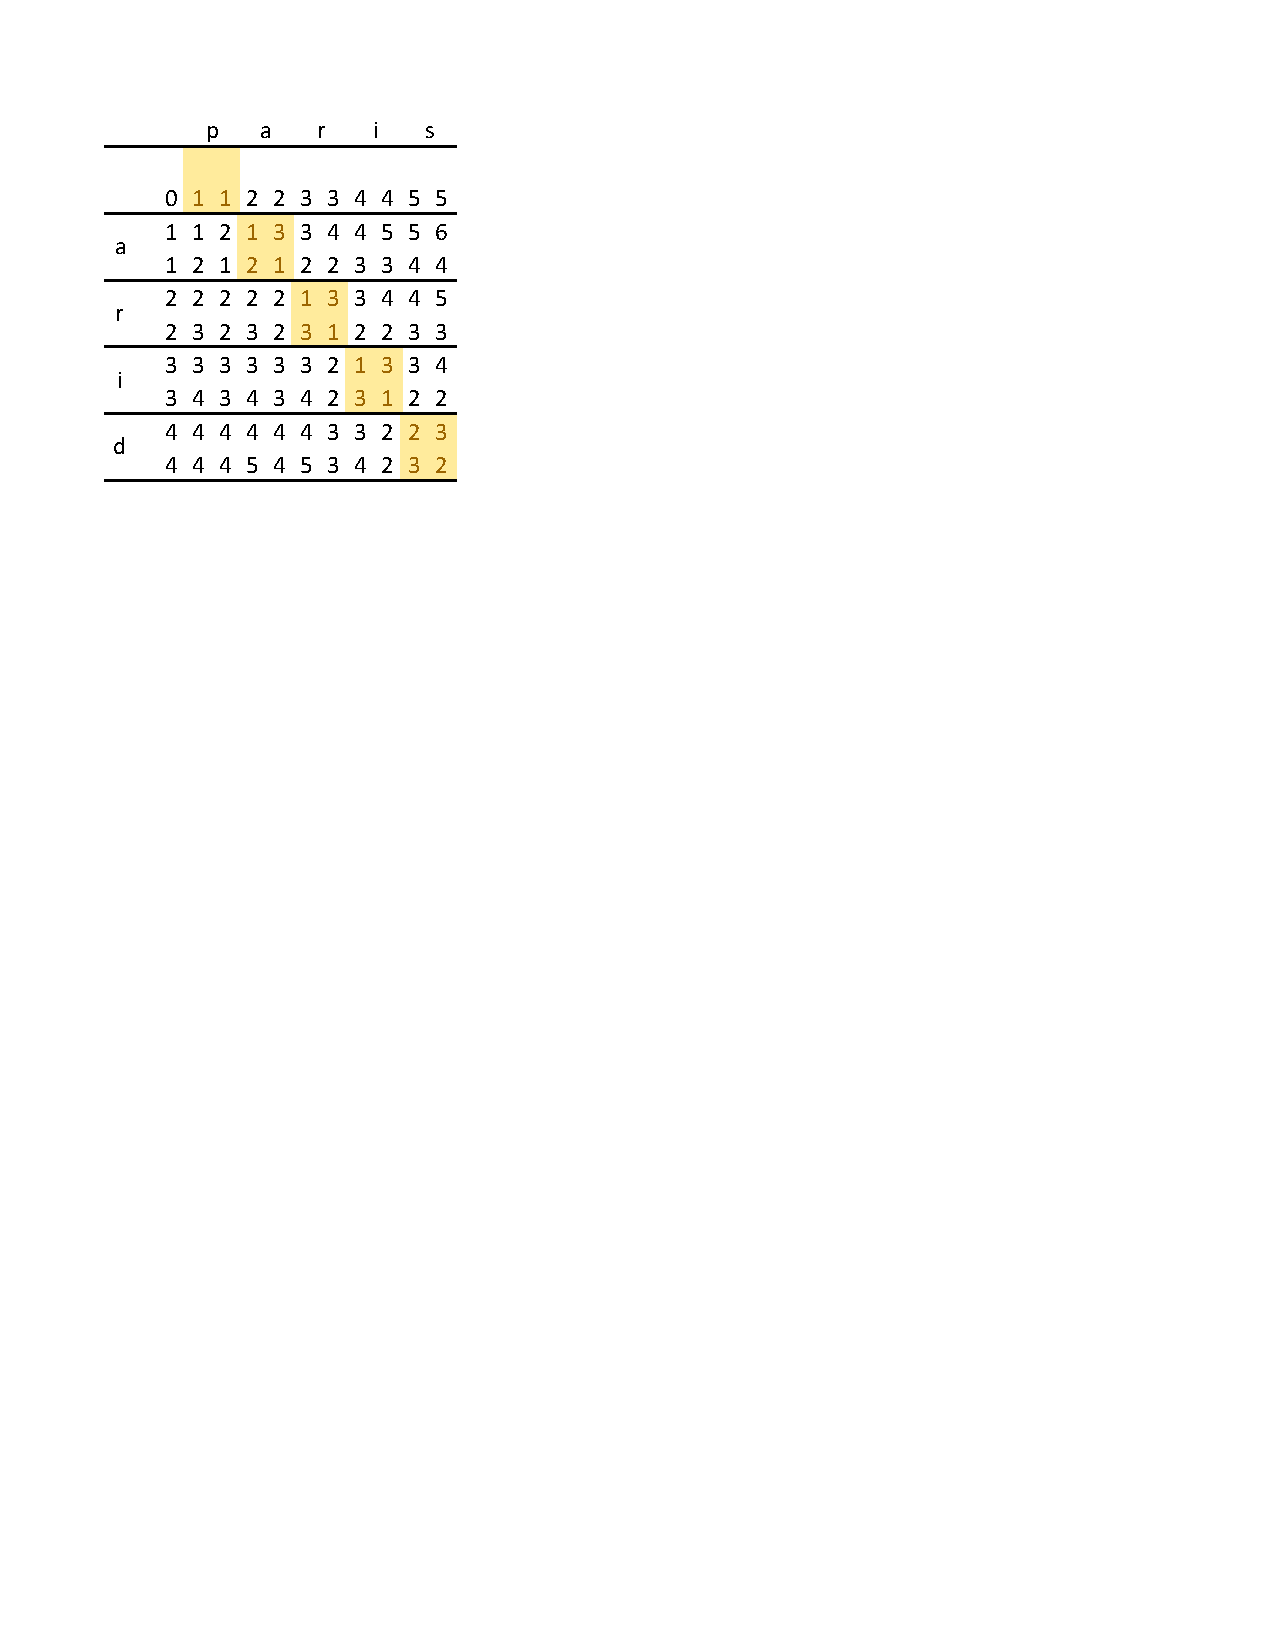
\includegraphics[width=3in]{Workbook1.pdf}
\caption{The yellow path shows the minimum edit distance path}
\label{distmatrix}
\end{center}
\end{figure}

\section{Problem 6}

\textbf{Consider the fragment of a positional index shown in homework problem 6. \\
The /k operator, word1 /k word2 finds occurrences of word1 within k words of word2 (on either side), where k is a positive integer argument. Thus k = 1 demands that word1 be adjacent to word2.}

\textbf{1. Describe the set of documents that satisfy the query Gates /2 Microsoft.}\\
Document 1: (Gates 3, Microsoft 1) \\
Document 3: (Gates 2, Microsoft 3)

\textbf{2. Describe each set of values for k for which the query Gates /k Microsoft returns a different set of documents as the answer.}\\
If we give /k the value of 1 and 5; \\
for /k = 1: Only document 3 will be returned.\\
for /k = 5: Documents, 1,2, and 3 will be returned.


\section{Problem 7: Project}
\subsection{Part 1}
\textbf{Construct a positional index and add support for Boolean proximity queries using the /k operator. That is, word1 /k word2 finds occurrences of word1 within k words of word2 (on either side), where k is a positive integer argument. Hint: use the algorithm from Figure 2.12 in the IIR textbook.}
\\
\\
The following code was used (python):
\lstinputlisting[language=Python]{q7p1.py}

\textbf{What does your code return for the file above and the query: schizophrenia /2 drug? How about schizophrenia /4 drug?}
\\
\textbf{schizophrenia /2 drug}: \\ $[(1, 3, 1), (2, 1, 2)]$ \\
This means we have two matches: \\
 a) In the document 1 (Doc1), schizophrenia is in position 3 and drug is in position 1. \\
 b) In the document 2 (Doc2), schizophrenia is in position 1 and drug is in position 2
\\
\textbf{schizophrenia /4 drug}: \\ $[(1, 3, 1), (2, 1, 2), (3, 5, 1)]$ \\
This means we have three matches: \\
 a) In the document 1 (Doc1), schizophrenia is in position 3 and drug is in position 1. \\
 b) In the document 2 (Doc2), schizophrenia is in position 1 and drug is in position 2 \\
 c) In the document 3 (Doc3), schizophrenia is in position 5 and drug is in position 1

\subsection{part 2}

\textbf{Modify the above algorithm to be directional. That is, the query word1 /k word2 must return occurrences of word1 strictly before word2, within k words. }
\\
The following code was used (python):
\lstinputlisting[language=Python]{q7p2.py}

\textbf{What does your code return for the file above and the query:}\\ \textbf{schizophrenia /2 drug}: \\ $[(2, 1, 2)]$ \\
This means we only have one match: \\
In the document 2 (Doc2), schizophrenia is in position 1 and drug is in position 2 

\section{Problem 8}
\textbf{Artificial intelligence (AI) and automation in general clearly improve the quality of our lives (think Google Scholar). However, in many cases, they also eliminate jobs (e.g., the self-driving car impacts the livelihood of taxi drivers). Most often, these negative side effects impact the people least prepared to recover. If you were a policy maker, how would you address this problem? Please describe your solution and explain one of its advantages, and one drawback.}

First of all, it should be mentioned that in addition to the improvement in the quality of life that automation brings, laborer jobs (blue-color worker) will also be replaced with more professional jobs. This means the importance of education will increase as well, and having more educated people in a society will be very beneficial in the long-term. 

Regarding the policymaking, I believe AI and automation will increase the country's GDP (gross domestic product). Having a wealthier country, we can help people that have been more affected to recover. By either helping them to get educated (if young) or even handing them salary without asking them to work (for older people). One advantage that this method has is that it will help people to get more educated. In the other hand, the disadvantages of this method are that it might increase laziness among some of the people.
\end{document}

